\chapter{Maquina de Vetores Suporte}\label{chp:LABEL_CHP_2}

%exemplo: 
%caso teste:
%classe:
%atributo


%\section{Definição}\label{sec:LABEL_CHP_2_SEC_A}
%silvana: icluir traducao parao portugues...
%silvana: sempre que usar termo em ingles, escrevê-lo em italico ({\em ...})
Maquina de Vetores de Suporte é uma classe de aprendizado de maquina que surgiu nos anos 90. Hoje em dia são usadas em diversas áreas como reconhecimento de escrita, bioinformática e mineração de dados.	Essencialmente trata-se de métodos de aprendizado supervisionado que podem ser usados para classificação binária, onde a partir de um conjunto de dados de treinamento a maquina aprende a classificar um novo exemplo como sendo de uma de duas classes; ou multi-classe, podendo classificar entre diversas classes. Para isso o problema é subdividido em problemas binários menores. Também é possível usar uma MVS para regressão quando você quer estimar uma valor ou probabilidade ao invés de uma classe. 
%silvana: caracterizar classificacao e regressao, binario e multi-classe
%Felipe: melhor?
%silvana: sim :)

Por simplicidade vou abordar aqui os classificadores binários, já que é preciso entender bem como ele funciona antes de entender os outros métodos. Sigo o fluxo de explicação abordado no livro \cite{art:LIVRO_SVM} que explica a teoria por tras da Maquina de Vetores de Suporte de forma bem didática.

\section{Superfícies de Decisão Lineares}
Uma forma simples de se criar um classificador é através de uma superfície de decisão linear. Dado um conjunto de dados $(\bar{x}_i,y_i)$ onde $\bar{x}_i \in \mathbb{R}^n$ são os parâmetros de cada exemplo e $y_i \in \{ -1,+1 \}$ é a classe que você deseja classificar definida como $+1$ ou $-1$. Se o conjunto for linearmente separável é possível criar uma superfície de decisão linear (reta, plano ou hiperplano) que separa esse conjunto de dados.

Uma vez encontrado o plano separador a classificação fica fácil. Se definirmos esse plano como $\bar{d}\cdot \bar{x} = \bar{d}\cdot \bar{c}$ onde $\bar{d}$ é o vetor ortogonal ao plano, $\bar{c}$ é o vetor de deslocamento de $\bar{d}$ e $\bar{x}$ são os pontos pertencentes a reta. Podemos classificar um ponto $\bar{\alpha}$ como pertencendo a uma classe usando uma função discriminante \ref{eq:LABEL_EQ_1} onde a classe é definida pelo sinal do resultado.

\begin{equation}
f(\bar{\alpha})=sgn((\bar{\alpha}-\bar{c})\cdot\bar{d})
    \label{eq:LABEL_EQ_1}
\end{equation}

\begin{figure}
  \centering
  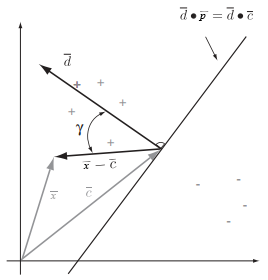
\includegraphics[width=0.4\textwidth]{imagens/svm_1.png}
  \captionsource{Classificação de um ponto $\bar{\alpha}$ por uma superfície de decisão linear}{\cite{art:LIVRO_SVM}}
  \label{fig:LABEL_FIG_1}
\end{figure}

%silvana: definir perceptron...
%silvana: Ok!
Como estamos assumindo que nossos dados são linearmente separáveis já sabemos qual a função discriminante, falta encontrar os parâmetros $\bar{c}$ e $\bar{d}$ que classificam corretamente esse conjunto de dados. Existem algumas formas de encontrar os parâmetros que definem essa superfície de decisão linear, um método próximo da maquina de vetores de suporte é o perceptron. O perceptron atribui valores aleatórios a $\bar{c}$ e $\bar{d}$ e classifica o conjunto de dados usando a função discriminante. A cada iteração, o perceptron corrige os valores de $\bar{c}$ e $\bar{d}$ para os dados que estiverem classificados de forma errada. Dessa forma se o conjunto de dados for linearmente separável o perceptron vai convergir para a superfície de decisão linear.

Essa superfície separa perfeitamente os exemplos usados no treinamento, mas pode ter muitos erros para classificar dados reais. Isso ocorre porque o perceptron não tem nenhum critério para saber se a superfície é boa ou ruim. Usando a figura \ref{fig:LABEL_FIG_2} como exemplo vamos supor que os pontos +* e -* não estavam no conjunto de treinamento e o perceptron chegou na linha pontilhada como superfície de separação. A linha preta seria mais adequada já que divide o espaço de forma mais justa reduzindo a chance de ter um ponto classificado errado.

\begin{figure}
  \centering
  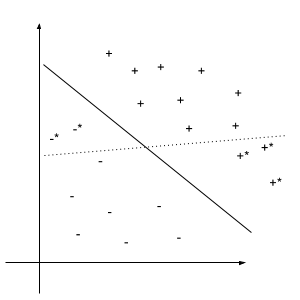
\includegraphics[width=0.4\textwidth]{imagens/svm_2.png}
  \caption{A linha preta representa a melhor separação e a linha pontilhada representa uma separação com maior chance de erro}
  \label{fig:LABEL_FIG_2}
\end{figure}

Para encontrar essa superfície precisamos definir hiperplanos de suporte e vetores de suporte. Hiperplanos de suporte são as superfícies que tangenciam os dados de cada classe que nos queremos separar. Esses hiperplanos devem ser paralelos e a nossa superfície de decisão ótima deve se encontrar no meio desses dois hiperplanos. Vetores de suporte são os pontos que pertencem a essas superfícies.
Podemos ver na figura \ref{fig:LABEL_FIG_3} que a superfície de decisão ótima vai ser encontrada quando a margem entre nossos hiperplanos de suporte for máxima.

\section{Classificadores de Margem Máxima}
Isso nos leva ao próximo conceito, classificadores de margem máxima. Essas técnicas tem como objetivo encontrar a superfície central entre dois conjuntos de dados (A linha preta, na figura anterior) para minimizar a chance de erro na classificação.

\begin{figure}
  \centering
  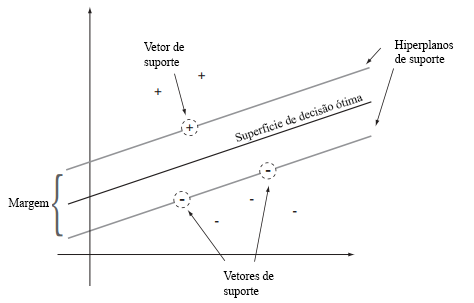
\includegraphics[width=0.7\textwidth]{imagens/svm_3.png}
  \captionsource{Superfície de decisão ótima e seus vetores e hiperplanos de suporte}{\cite{art:LIVRO_SVM}}
  \label{fig:LABEL_FIG_3}
\end{figure}

Como estamos procurando a margem máxima dado um conjunto de margens possíveis faz sentido abordar o problema como um problema de otimização.

Formalmente problemas de otimização são definidos como: $\underset{\bar{x}}{min}\phi(\bar{x})$ dado que $h_i(\bar{x})\ge c_i$ $\forall \bar{x} \in \mathbb{R}^n$. Onde $\phi: \mathbb{R}^n\rightarrow \mathbb{R}$ é a função objetivo que se quer minimizar e $h_i:\mathbb{R}^n\rightarrow\mathbb{R}$ é o limitante da função com limite $c_i$

Podemos então traduzir o problema de separar o conjunto de dados em um problema de otimização onde o objetivo é maximizar a distancia entre as superfícies de suporte. As superfícies de suporte são definidas como hiperplanos paralelos que tangenciam os conjuntos de dados de cada classe. E vetores de suporte são pontos pertencentes a essas superfícies. Assim o que nós queremos é a função da superfície de decisão ótima $\bar{w}^*\cdot\bar{x}=b^*$ onde a projeção entre os vetores de suporte $m^*=|\bar{x}_p - \bar{x}_q|cos\gamma$ é máximo como podemos ver na figura \ref{fig:LABEL_FIG_4}. 

\begin{figure}
  \centering
  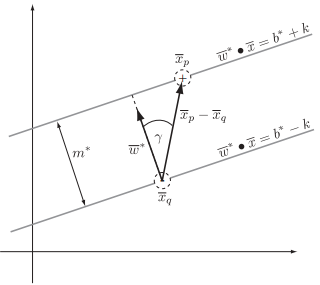
\includegraphics[width=0.6\textwidth]{imagens/svm_4.png}
  \captionsource{Calculando a margem $m^*$ entre os planos de suporte}{\cite{art:LIVRO_SVM}}
  \label{fig:LABEL_FIG_4}
\end{figure}

Para prosseguir nossos cálculos vamos precisar rescrever $m^*$ como: $\frac{2k}{|\bar{w}^*|}$.

\begin{equation}
m^* = |\bar{x}_p-\bar{x}_q|cos\gamma
    \label{eq:LABEL_EQ_2}
\end{equation}

\begin{equation}
= \frac{\bar{w}^*\cdot(\bar{x}_p-\bar{x}_q)}{|\bar{w}^*|}
    \label{eq:LABEL_EQ_3}
\end{equation}

\begin{equation}
= \frac{\bar{w}^*\cdot\bar{x}_p-\bar{w}^*\cdot\bar{x}_q}{|\bar{w}^*|}
    \label{eq:LABEL_EQ_4}
\end{equation}

\begin{equation}
= \frac{(b^*+k)-(b^*-k)}{|\bar{w}^*|}
    \label{eq:LABEL_EQ_5}
\end{equation}

\begin{equation}
= \frac{2k}{|\bar{w}^*|}
    \label{eq:LABEL_EQ_6}
\end{equation}

\begin{equation}
\begin{split}
m^* &= |\bar{x}_p-\bar{x}_q|cos\gamma\\
    &= \frac{\bar{w}^*\cdot(\bar{x}_p-\bar{x}_q)}{|\bar{w}^*|}\\
    &= \frac{\bar{w}^*\cdot\bar{x}_p-\bar{w}^*\cdot\bar{x}_q}{|\bar{w}^*|}\\
    &= \frac{(b^*+k)-(b^*-k)}{|\bar{w}^*|}\\
    &= \frac{2k}{|\bar{w}^*|}
\end{split}
\end{equation}

Queremos $m^*$ máximo mas para facilitar nossos cálculos mais a frente vamos reescrever nossa função objetivo como:

\begin{equation}
\begin{split}
m^* &= max \frac{2k}{|\bar{w}|} \\
    &= min \frac{|\bar{w}|}{2k} \\
    &= min \frac{|\bar{w}|^2}{2k}  \\
    &= min \frac{1}{2k} \bar{w}\cdot\bar{w}  \\
    &= min \frac{1}{2} \bar{w}\cdot\bar{w}
\end{split}
\end{equation}

Nossas restrições podem ser escritas como:
%Felipe: essa notação ta certa o tal que? precisa de uma chave aí?
\begin{equation}
\begin{split}
\bar{w}^*\cdot\bar{x}_i \ge b^*+k \quad \forall (\bar{x}_i,y_i)\in D \quad | \quad y_i=+1 \\
\bar{w}^*\cdot\bar{x}_i \le b^*-k \quad \forall (\bar{x}_i,y_i)\in D \quad | \quad y_i=-1 \\
\bar{w}^*\cdot\bar{x}_i \ge 1+b \quad \forall (\bar{x}_i,y_i)\in D \quad | \quad y_i=+1 \\
\bar{w}^*\cdot(-\bar{x}_i) \ge 1-b \quad \forall (\bar{x}_i,y_i)\in D \quad | \quad y_i=-1 \\
\bar{w}^*\cdot(y_i\bar{x}_i) \ge 1+y_i b \quad \forall (\bar{x}_i,y_i)\in D
\end{split}
\end{equation}

Assim um classificador por margem máxima fica definido como: Dado um conjunto de dados linearmente separáveis $D=(\bar{x}_i,y_i) \subseteq \mathbb{R}^n\times\{+1,1\}$, podemos encontrar a superfície máxima de separação, $\bar{w}^*\cdot\bar{x}=b^*$, otimizando o problema $min\phi(\bar{w},b)=\underset{\bar{w},b}{min}\frac{1}{2}\bar{w}\cdot\bar{w}$ sujeito as restrições de $\bar{w}^*\cdot(y_i\bar{x}_i) \ge 1+y_i b \quad \forall (\bar{x}_i,y_i)\in D$.\par

Uma maquina de vetores de suporte é o problema dual do classificador de margem máxima. Podemos entender um problema dual como uma versão análoga do problema onde invés de encontrar o vetor que define a superfície de separação $w$, queremos encontrar o conjunto de valores de $a$ do qual podemos inferir $w$. Para resolver esse problema dual utilizamos a técnica dual Lagrangiana. Essa técnica pode ser vista nos trabalhos de \cite{art:LIVRO_SVM} e \cite{art:LIVRO_KAA}.

O método de otimização Lagrangiana reescreve um problema de otimização da forma:
\begin{equation}
\underset{\bar{x}}{min}\phi(\bar{x}) \quad \text{dado que} \quad h_i(\bar{x})\ge c_i
\end{equation}
como:
\begin{equation}
\underset{\bar{\alpha}}{max} \underset{\bar{x}}{min} L(\bar{\alpha},\bar{x}) = \underset{\bar{\alpha}}{max} \underset{\bar{x}}{min}\bigg(\phi(\bar{x})-\sum_{i=1}^{l}\alpha_i g_i(\bar{x})\bigg)
    \label{eq:LABEL_EQ_7}
\end{equation}
dado que
\begin{equation}
\alpha_i\ge0
    \label{eq:LABEL_EQ_8}
\end{equation}
Encontrados os valores máximo de $a^*$ e minimo de $x^*$ a solução do problema dual vai ser o mesmo do problema primal contanto que as seguintes condições se apliquem:

\begin{equation}
\begin{split}
\frac{\partial L}{\partial \bar{x}}(\bar{\alpha}^*,\bar{x})&=\bar{0}, \\
\alpha_i^*g_i(\bar{x}^*)&=\bar{0}, \\
g_i(\bar{x}^*)&\ge\bar{0} , \\
\bar{\alpha}_i^*(\bar{x}^*)&\ge\bar{0} 
\end{split}
\end{equation}

Essas condições são conhecidas como as condições de Karush-Kuhn-Tucker ou KKT e podemos usar elas para reescrever nosso problema dependendo somente de $\bar{\alpha}$ facilitando nossa busca. Agora podemos aplicar essa técnica no nosso problema de margem máxima, escrevemos nossa função lagrangiana como:

\begin{equation}
\begin{split}
L(\bar{\alpha},\bar{w},b) &=\phi(\bar{w},b) -  \sum_{i=1}^{l}\alpha_i g_i (\bar{w},b) \\
 &=\frac{1}{2}\bar{w}\cdot\bar{w} - \sum_{i=1}^{l}\alpha_i (y_i(\bar{w}\cdot \bar{x}_i -b)-1) \\
 &=\frac{1}{2}\bar{w}\cdot\bar{w} - \sum_{i=1}^{l}\alpha_i y_i \bar{w}\cdot \bar{x}_i + b \sum_{i=1}^{l}\alpha_i y_i + \sum_{i=1}^{l}\alpha_i\\
\end{split}
\end{equation}

Aplicando as KKTs chegamos no nosso classificador de margem máxima dual:
\begin{equation}
    \underset{\bar{\alpha}}{max} \phi' (\bar{\alpha}) = \underset{\bar{\alpha}}{max} \Bigg( \sum_{i=1}^{l}\alpha_i - \frac{1}{2}\sum_{i=1}^{l}\sum_{j=1}^{l}\alpha_i \alpha_j y_i y_j \bar{x}_i\cdot \bar{x}_j \Bigg)
    \label{eq:EQ_Treinador_1}
\end{equation}
dado que:
\begin{equation}
    \sum_{i=1}^{l}\alpha_i y_i = 0 \quad \text{e} \quad \alpha_i \ge 0 \forall \quad i \in \{1,l\}
    \label{eq:restricoes}
\end{equation}

Uma vez encontrado nosso $\bar{\alpha}^*$ ótimo podemos classificar um novo ponto $\bar{x}$ com a formula:

\begin{equation}
    f(\bar{x}) = sgn\Bigg(
        \sum_{i=1}^{l} \alpha_i^*y_i\bar{x}_i\cdot\bar{x}
        -b^*
    \Bigg)
    \label{eq:EQ_Classificador_1}
\end{equation}

\begin{equation}
    b^* = \sum_{i=1}^{l} \alpha_i^*y_i\bar{x}_i\cdot\bar{x}_{sv+}
        -1
    \Bigg)
    \label{eq:EQ_B_1}
\end{equation}

Onde $b^*$ representa a distancia da origem do plano, $\alpha_i^*=0$ implica que $\bar{x}_i$ não influencia no resultado, $\alpha_j^*> 0$ implica que $\bar{x}_j$ é um vetor de suporte e $\bar{x}_{sv+}$ é um vetor de suporte positivo qualquer.


\section{O Truque do Kernel}
Com isso conseguimos uma maquina de vetores de suporte linear. Acontece que poucos conjuntos de dados na pratica são linearmente separáveis. Para aplicar nossa maquina em um conjunto de dados que não seja linearmente separáveis precisamos projeta-los de forma que fiquem linearmente separáveis, como na figura \ref{fig:LABEL_FIG_5}

\begin{figure}
  \centering
  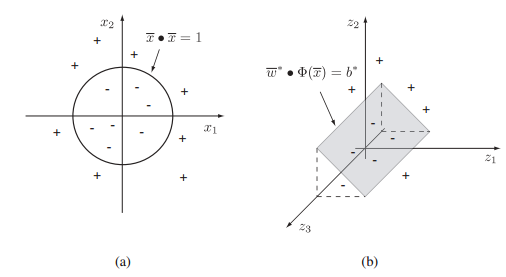
\includegraphics[width=1\textwidth]{imagens/svm_5.png}
  \captionsource{Em (a) não é possível separar os conjuntos de forma linear, mas transformando os dados em $\mathbb{R}^2\rightarrow \mathbb{R}^3$ em (b) conseguimos separa-los linearmente}{\cite{art:LIVRO_SVM}}
  \label{fig:LABEL_FIG_5}
\end{figure}

Para Isso precisamos escolher funções de projeção $ \phi:\mathbb{R}^n\rightarrow\mathbb{R}^m$. Assim passamos todos nossos exemplos para um espaço de dimensão maior na esperança que nesse espaço eles possam ser linearmente separáveis. 

Podemos ver nas equações de treinamento \ref{eq:EQ_Treinador_1} e classificação \ref{eq:EQ_Classificador_1} que sempre é avaliado o produto de dois conjuntos de dados $\bar{x}_i\cdot\bar{x}_j$, então podemos substituir $\phi(\bar{x}_i) \cdot \phi ( \bar{x}_j )$ por $k(\bar{x}_i,\bar{x}_j)$ de forma que que seja mais simples que o produto de $\phi(\bar{x})$.

Na figura \ref{fig:LABEL_FIG_5} $\phi(\bar{x})=(x_1^2,x_2^2,\sqrt{2}x_1x_2)$ e podemos simplificar seu produto:

\begin{equation}
\begin{split}
\phi(\bar{x})\cdot \phi(\bar{y}) &= (x_1^2,x_2^2,\sqrt{2}x_1x_2) \cdot (y_1^2,y_2^2,\sqrt{2}y_1y_2) \\
&=x_1^2y_1^2+x_2^2y_2^2+2x_1x_2y_1y_2 \\
&=(x1y1+x2y2)(x1y1+x2y2) \\
&=(\bar{x}\cdot\bar{y})(\bar{x}\cdot\bar{y}) \\
&=(\bar{x}\cdot\bar{y})^2
\end{split}
\end{equation}

Chamamos essa simplificação de Truque de Kernel. Existe um estudo grande sobre Kernels validos e uma seria de restrições que uma função tem que cumprir para ser considerada um Kernel válido. Não me aprofundarei nesse assunto aqui. Muitos desses kernels possuem uma variável livre que deve ser adaptada ao conjunto de dados estudado podendo influenciar na sua precisão. Alguns kernels populares e suas variáveis livres são:
\begin{table}
    \centering
    \caption{Kernels Populares e suas váriaveis livres}
    \begin{tabular}{c|c|c}
            Kernel & Função & Parametros Livres \\ \hline
        Kernel Linear & $k(\bar{x},\bar{y})=\bar{x}\cdot\bar{y}$ & nenhum \\
        Kernel Homogeneo Polinomial & $k(\bar{x},\bar{y})=(\bar{x}\cdot\bar{y})^2$ & $d\ge2$ \\
        Kernel Não-Homogeneo Polinomial & $k(\bar{x},\bar{y})=(\bar{x}\cdot\bar{y}+c)^2$ & $d\ge2, c > 0$ \\
        Kernel Gaussiano & $k(\bar{x},\bar{y})=e^{-\big(\frac{|\bar{x}-\bar{y}|^2}{2\sigma^2}\big)}$ & $\sigma>0$ \\ \hline
    \end{tabular}
    %\caption{Kernels Populares e suas váriaveis livres}
    \label{tab:Kernels}
\end{table}

Para transformar nossa maquina de vetor de suporte linear em um não linear apenas substituímos $\phi(\bar{x}_i) \cdot \phi ( \bar{x}_j )$ por $k(\bar{x}_i,\bar{x}_j)$ em \ref{eq:EQ_Treinador_1}, \ref{eq:EQ_Classificador_1} e \ref{eq:EQ_B_1}.

Treinador:
\begin{equation}
    \bar{\alpha}^* = \underset{\bar{\alpha}}{argmax}{\phi}'(\bar{\alpha}) =\underset{\bar{\alpha}}{argmax} \Bigg( \sum_{i=1}^{l}\alpha_i - \frac{1}{2}\sum_{i=1}^{l}\sum_{j=1}^{l}\alpha_i \alpha_j y_i y_j k(\bar{x}_i,\bar{x}_j) \Bigg)
    \label{eq:EQ_Treinador_2}
\end{equation}

Classificador:
\begin{equation}
    f(\bar{x}) = sgn\Bigg(
        \sum_{i=1}^{l} \alpha_i^*y_i k(\bar{x}_i,\bar{x})
        -b^*
    \Bigg)
    \label{eq:EQ_Classificador_2}
\end{equation}
\begin{equation}
    b^* = \sum_{i=1}^{l} \alpha_i^*y_i k(\bar{x}_i,\bar{x}_{sv+})
        -1
    \Bigg)
    \label{eq:EQ_B_2}
\end{equation}

\section{Margem Flexível}
Conjuntos reais de dados possuem ruídos, e pontos anormais podem distorcer e piorar muito a performance de uma uma maquina de vetor de suporte. As maquinas vistas até agora são considerados com margem rígida, mas também existem máquinas de vetor de suporte que ignoram certos pontos dentro de um ruído considerados com margem flexível.

\begin{figure}
  \centering
  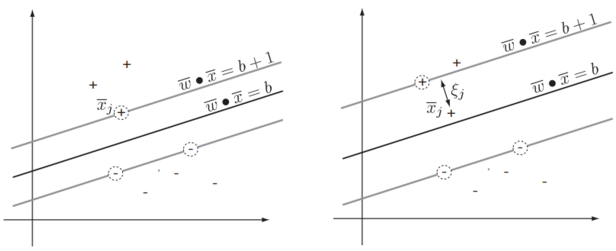
\includegraphics[width=1\textwidth]{imagens/svm_6.png}
  \captionsource{No exemplo da direita ignoramos $\bar{x}_j$ que pode ser considerado ruído}{\cite{art:LIVRO_SVM}}
  \label{fig:LABEL_FIG_6}
\end{figure}

Para isso escolhemos uma constante $C$ que atribuímos como um peso para os erros. No problema primal definimos $C$ como $\underset{\bar{w},\bar{\epsilon},b}{min}\phi(\bar{w},\bar{\epsilon},b) = \frac{1}{2}\bar{w}^*\cdot\bar{w}^* + C\sum_{i=1}^l \epsilon_i^*=m^*$ de forma que quanto maior $C$ maior o peso dos erros, mais próximo a margem flexível fica da margem rígida. Um $C$ menor permite mais erros fazendo com que a margem cresça e se distancie da margem rígida. No problema dual esse limite aparece como: $0\le \alpha_i \le C$

\section{Implementação}
Com isso definimos uma maquina de vetor de suporte bem robusto capaz de classificar conjuntos de dados não lineares e suscetíveis a ruídos. A complexidade de implementação de uma MVS consiste na dificuldade de se achar o valor máximo de $\bar{\alpha}$ existem alguns algoritmos diferentes para se chegar nesse resultado, alguns deles descritos em \cite{art:LIVRO_SVM} são:

%Felipe No livro está Gradient Ascent, não sei se essa tradução está boa
\subsection{Gradiente Ascendente}
O gradiente de um vetor é um vetor que aponta para a direção onde a função cresce naquele ponto. Dessa forma podemos calcular o gradiente de $\bar{\alpha}$ em um ponto aleatório e incrementar os valores de $\bar{\alpha}$ pelo gradiente. Sabemos que chegamos no máximo local quando o gradiente for $0$, ou quando a diferença de $\bar{\alpha}$ entre as iterações é aproximadamente $0$. Nesse ponto temos o valor ótimo de $\bar{\alpha}$. Apesar de não considerarmos $b$ nessa implementação seu valor pode ser encontrado a partir de $\bar{\alpha}$. Calculando o gradiente do nosso treinador encontrado em \ref{eq:EQ_Treinador_2} encontramos a equação \ref{eq:Gradiente}.

\begin{equation}
    \triangledown_i {\phi}'(\bar{\alpha}) = 1-y_i\sum_{j=1}^ly_j\alpha_jk(\bar{x}_j,\bar{x}_i)
    \label{eq:Gradiente}
\end{equation}
Não temos garantia que o tamanho do gradiente não seja maior que a distancia até o ponto ótimo por devemos incluir uma taxa de aprendizado $\eta$ multiplicado pelo gradiente, valores comuns de $\eta$ variam na faixa de $[0,1]$. Como o máximo da dual lagrangiana é único podemos garantir que o algoritmo vai convergir dado um $\eta$ pequeno o suficiente.

\begin{algorithm}
\label{alg:gradiente}
\caption{Algoritmo Gradiente Ascendente}
\begin{algorithmic}
\STATE $\eta>0$
\STATE $\bar{\alpha} \leftarrow \bar{0}$
\REPEAT
\STATE $\bar{\alpha_{old}} \leftarrow \bar{\alpha}$
\FOR{$i=1$ to $l$}
\STATE $\alpha_i \leftarrow a_i + \eta \triangledown_i {\phi}'(\bar{\alpha})$
\ENDFOR
\UNTIL{$\bar{\alpha}-\bar{\alpha_{old}}\approx \bar{0}$}
\RETURN $(\bar{\alpha},b)$
\end{algorithmic}
\end{algorithm}

\subsection{Algoritmo Kernel-Adatron} \label{sec:kaa}
O problema do Gradiente Ascendente é que ele ignora as restrições de otimização definidas em \ref{eq:restricoes}, não considera o valor de $b$ e não considera uma margem flexível. O algoritmo Kernel-Adatron resolve esses problemas. Em \cite{art:LIVRO_KAA} é explicado que a primeira restrição, $\sum_{i=1}^{l}\alpha_i y_i = 0$, só é necessária para restringir o valor de $b$ no ponto máximo. Ao fixar o valor de $b$ em zero podemos abrir mão dessa restrição. O valor de $b$ é usado para encontrar o deslocamento da origem da nossa superfície de decisão de forma que fixando ele em zero nos limitamos a hiperplanos que cruzem a origem no espaço de projeção. De acordo com Campbell, na pratica essa é uma generalização não prejudica os resultados quando estamos tratando de um espaço de muitas dimensões. Assim ficamos com as restrições $\alpha_i \ge 0$ e $\alpha_i \le C$ que pode ser facilmente implementado. Podemos ver o algoritmo descrito em \ref{alg:KAA}.

\begin{algorithm}
\label{alg:KAA}
\caption{Algoritmo Kernel-Adatron}
\begin{algorithmic}
\STATE $D = \{(\bar{x_i},y_1)...(\bar{x_i},y_1)\} \subset \mathbb{R}^{n}\times \{+1,-1\}$
\STATE $\eta>0$
\STATE $C>0$
\STATE $b=0$
\STATE $\bar{\alpha} \leftarrow \bar{0}$
\REPEAT
\STATE $\bar{\alpha_{old}} \leftarrow \bar{\alpha}$
\FOR{$i=1$ to $l$}
\STATE $\alpha_i \leftarrow min\big\{C,max\big\{0,\alpha_i + \eta-\eta y_i \sum_{j=1}^l y_j \alpha_j k(\bar{x}_j,\bar{x}_i))\big\}\big\}$
\ENDFOR
\UNTIL{$\bar{\alpha}-\bar{\alpha_{old}}\approx \bar{0}$}
\RETURN $(\bar{\alpha},b)$
\end{algorithmic}
\end{algorithm}

\subsection{Quadratic Program Solver}
Como a forma de se encontrar os valores de $\bar{\alpha}$ é um problema de otimização existem métodos genericos de otimização que ajudam nessa tarefa um deles é o \emph{Quadratic Program Solver}, um algoritmo que encontra os valores de um parâmetro que minimizam uma função dado um conjunto de restrições. Varias bibliotecas implementam esse algoritmo de forma que seria possivel resolver a SVM sem ter que implementar o algoritmo de otimização.
\subsection{SMO: Sequential Minimal Optimization}
Em vez de tentar encontrar todos os valores de $\alpha$ de uma vez o \emph{Sequential Minimal Optimization} escolhe dois pontos de treinamento, otimiza eles e vê se as restrições de KKT são válidas para o resto do conjunto de treinamento, caso contrário escolhe outros dois pontos e continua o algoritmo. Os pontos escolhidos são sempre de forma que um ponto respeite as restrições e o maior violador das restrições. Dessa forma é possível provar que o algoritmo vai convergir. Isso permite uma serie de otimizações mais complexas em cima das formulas vistas de forma que o calculo final fique mais simples e econômico.


%aloisio: passar para o capítulo 4
\subsection{Escolhido: Kernel-Adatron}
O algoritmo que acabei escolhendo foi o Kernel-Adatron, sua implementação é só um pouco mais complexa que o de incremento de gradiente e ainda tem um fluxo fácil de compreender. Não escolhi o \emph{Quadratic Program Solver} pois mudaria o foco do projeto para um algoritmo mais genérico de otimização. Apesar de o SMO ser o algoritmo mais usado nos artigos em que me baseei achei que seria interessante implementar primeiro o Kernel-Adatron já que seria mais fácil de entender como o algoritmo está convergindo o que as variáveis representam no resultado final. Além disso por o Kernel-Adatron ser um algoritmo mais custoso espero um ganho mais significativo da versão sequencial para a paralela, diferente do SMO que é um algoritmo otimizado para a execução sequencial eu teria de desfazer alguns de suas otimizações para funcionar de forma paralela.